\documentclass[12pt]{article}

\usepackage{graphicx,amsmath,textcomp,caption,subcaption,cite}
\usepackage[round]{natbib}
\usepackage[margin=2cm]{geometry}
%\usepackage[subtle]{savetrees}
\linespread{1.1}
\bibliographystyle{plainnat}
\title{
ENGN1218 Introduction to Electronics\\
Full-wave Rectifier Analysis\\
}
\author{
\and Paul Apelt, u5568225
\and Thomas Hale, u5567957
\and School of Engineering, ANU 
}
\begin{document}
\maketitle

\begin{abstract}
A diode-bridge full wave power rectifier circuit was designed and constructed. The aim was to achieve a 12V DC output with 10\% tolerance. A theoretical analysis of two types of diode-bridge full-wave rectifiers---with and without a capacitor---was conducted, and results confirmed using a computer simulation. The construction process was documented, and all output parameters measured. The aim was successfully achieved, with all output parameters matching the predicted values within an acceptable error bound.
\end{abstract}

\section{Introduction}
\label{sec:int}
Most forms of power are supplied in the form of AC current.As most electronics devices and systems require DC current it is necessary that there be a means to convert AC to DC. Power rectifier circuits allow this and function using diodes, which ideally only allow the passage of current in one direction - typically the positive direction.

There are several types of rectifier circuits that can be used to convert from AC to DC current but only the full wave rectifier or bridge rectifier will be discussed in this report. The bridge rectifier circuit---as per Figure~\ref{fig:cap}---is designed such that current during both the negative and positive cycles pass through the load site in the same direction, which means that the voltage across the load site is always of the same sign. Although this configuration of diodes succeeds in inverting the voltage in the negative cycle, the voltage is not the constant DC voltage that is desired. In order to reduce this voltage variation a capacitor is added in series with the load site. The capacitor charges when the voltage from the source is increasing and discharges when the voltage from the source is decreasing, thus smoothing the output waveform. 

\section{Theoretical Analysis}
\label{sec:the}
Two versions of a full-wave rectifier circuit were analysed, with and without a smoothing capacitor, schematics shown in Figures \ref{fig:cap} and \ref {fig:nocap} respectively.
\begin{figure}[h!]
\centering
\begin{subfigure}[b]{0.45\textwidth}
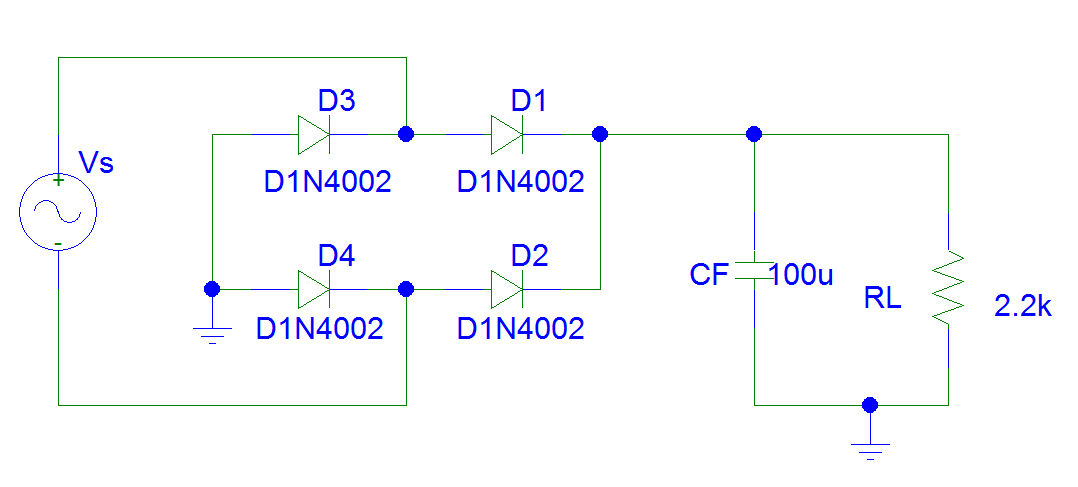
\includegraphics[width=\textwidth]{rekt_cap}
\caption{Full-wave rectifier with a capacitor filter.}
\label{fig:cap}
\end{subfigure}
\qquad
\begin{subfigure}[b]{0.45\textwidth}
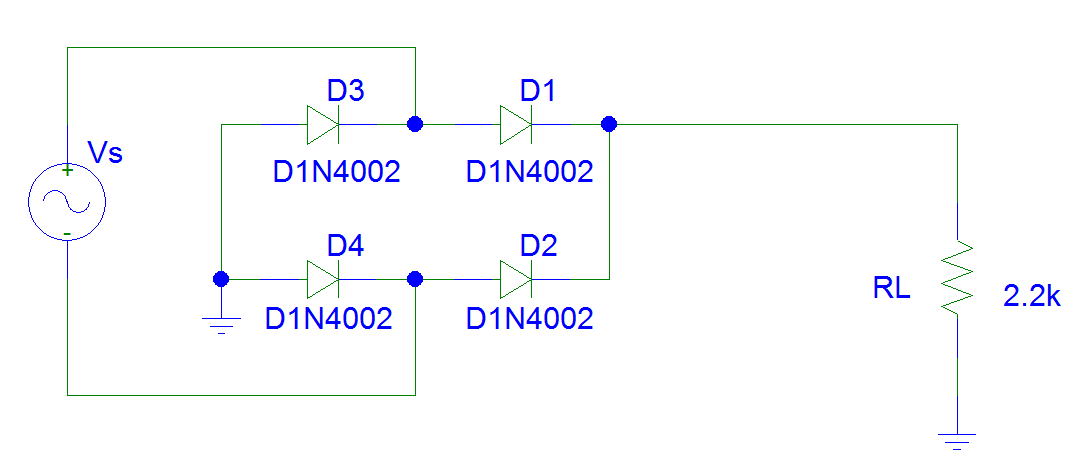
\includegraphics[width=\textwidth]{rekt_nocap}
\caption{Full-wave rectifier without a capacitor filter.}
\label{fig:nocap}
\end{subfigure}
\caption{Schematics.}
\label{fig:sch}
\end{figure}

To predict the output of the rectifier circuit, formulas from the lecture notes were used \citep{lecture}. The value for the input voltage $V_{in}$\footnote{Unless explicitly stated otherwise, all AC voltage values are peak-to-peak.} was taken to be equal to the actual output of the transformer used during testing (see Section~\ref{sec:imp}). The output voltage of a rectifier without a capacitor filter was calculated in Equation~\ref{eq:nocap}, and the voltage ripple and DC voltage output of the rectifier with a smoothing capacitor---in Equations \ref{eq:cap} and \ref{eq:capdc} respectively.
\begin{align}
\begin{split}
V_{out}&=V_{in}-2\times0.7\\
&=18.8-1.4\\
&=17.4\mathrm{V}
\label{eq:nocap}
\end{split}
\end{align}

Note that in the above case, in the absence of the smoothing capacitor, $V_r=V_{out}$. The addition of a capacitor has no effect on the output peak voltage, but decreases ripple.
\begin{align}
\begin{split}
  \begin{cases}
  V_{r}=\frac{V_{DC}}{2f R_L C}\\
  V_{DC}=V_{out}-\frac{1}{2}V_r
  \end{cases}
  \Leftrightarrow
  V_{r}&=\frac{2V_{out}}{4fR_LC+1}\\
  &=\frac{2\times17.4}{4\times50\times2.2\times10^{3}\times10^{-4}+1}\\
  &=0.773\mathrm{V}
\label{eq:cap}
\end{split}
\end{align}
\begin{align}
  \begin{split}
    V_{DC}&=V_{out}-\frac{1}{2}V_r\\
    &=17.4-\frac{0.773}{2}\\
    &=17.01
  \end{split}
  \label{eq:capdc}
\end{align}
\section{Simulation}
\label{sec:sim}
\section{Implementation}
\label{sec:imp}
\section{Discussion}
\label{sec:dis}
\section{Conclusion}
\label{sec:con}
\bibliography{electronics.bib}
\end{document}
